\documentclass[12pt,a4paper]{article}

\usepackage[utf8]{inputenc}
\usepackage[T1]{fontenc}
\usepackage{parskip}
\usepackage{amsmath, amssymb, graphicx}
\usepackage{tcolorbox}
\usepackage{fancyhdr}
\graphicspath{{/Users/econhead/NOTES/Microeconomics/MicroClassNotes/20_10_2024/Figures}}
\setlength{\headheight}{15.6pt}
\pagestyle{fancyplain}
\fancyhead[L]{Laxman Singh}
\fancyhead[R]{\today}
\usepackage{float}
\floatstyle{boxed}
\restylefloat{figure}

\author{Laxman Singh}
\date{\today}
\title{Externalities}

\begin{document}
 \section*{\underline{Externalities}}
 \subsection*{\underline{Pure Exchange Economy with Externalities}}  
 Set of all Feasible allocations;
 \begin{equation*}
     \mathcal{F}= \{\left( (x_{1},y_{1}),(x_{2},y_{2}) \right) \in \mathbb{R}^2_{+} \times \mathbb{R}^2_{+} | x_{1}+x_{2}=\omega_{1}^X + \omega^X_{2} , y_{1}+y_{2}= \omega^Y_{1}+\omega^Y_{2} \}
 \end{equation*}  
 
 Alternative Definition of feasible allocations;
 \begin{equation*}
    \mathcal{F}= \{\left( (x_{1},y_{1}) , (x_{2},y_{2}) \right) \in \mathbb{R}^2_{+} \times \mathbb{R}^2_{+} | x_{1}+x_{2}\leq \omega_{1}^X + \omega^X_{2} , y_{1}+y_{2}\leq \omega^Y_{1}+\omega^Y_{2}\}
 \end{equation*}
  
 In an Environment with Externalities;
 \begin{equation*}
    \begin{split}
        u_{1}: \mathbb{R}^2_{+} \times \mathbb{R}^2_{+} \quad u_{1}(x_{1},y_{1},x_{2},y_{2})\\
        u_{2}: \mathbb{R}^2_{+} \times \mathbb{R}^2_{+} \quad u_{2}(x_{1},y_{1},x_{2},y_{2})  
    \end{split}
    \end{equation*}
Endowments of the two individuals are;
\begin{equation*}
    \left( \omega_{1}^X, \omega_{1}^Y \right) \quad \text{and} \quad \left( \omega_{2}^X , \omega_{2}^Y \right)  
\end{equation*} 
\subsubsection*{Question 1}
Find the set of all Pareto Efficient allocations of the following economy;
   \begin{align*}
       u_{1}(x_{1},y_{1},x_{2},y_{2})= 3x_{1}+2y_{1}+2x_{2} \qquad (2,0) \\
       u_{2}(x_{1},y_{1},x_{2},y_{2})= 2x_{2}+3y_{2}+2y_{1} \qquad (0,2)\\
   \end{align*}
   We first start with finding the adjusted utility functions using the feasability constraints;
  \begin{align*}
    u_{1}^{ADJ}(x_{1},y_{1})=u_{1}(x_{1},y_{1},2-x_{1},2-y_{1})= x_{1}+2y_{1}+4\\
    u_{2}^{ADJ}(x_{2},y_{2})=u_{1}(x_{2},y_{2},2-x_{2},2-y_{2})= 2x_{2}+y_{2}+4\\
  \end{align*}
  Now we can plot the indifference curves in the edgeworth box and find the set of all Pareto Efficient allocations;
  
  \begin{equation*}
      PE= \{\left( (x_{1},y_{1}),(x_{2},y_{2}) \right) \in \mathcal{F} | \ x_{1}=0 \vee y_{1}=2\} 
  \end{equation*}    
  
  \begin{center}
    \begin{figure}[ht!]
        \centering
        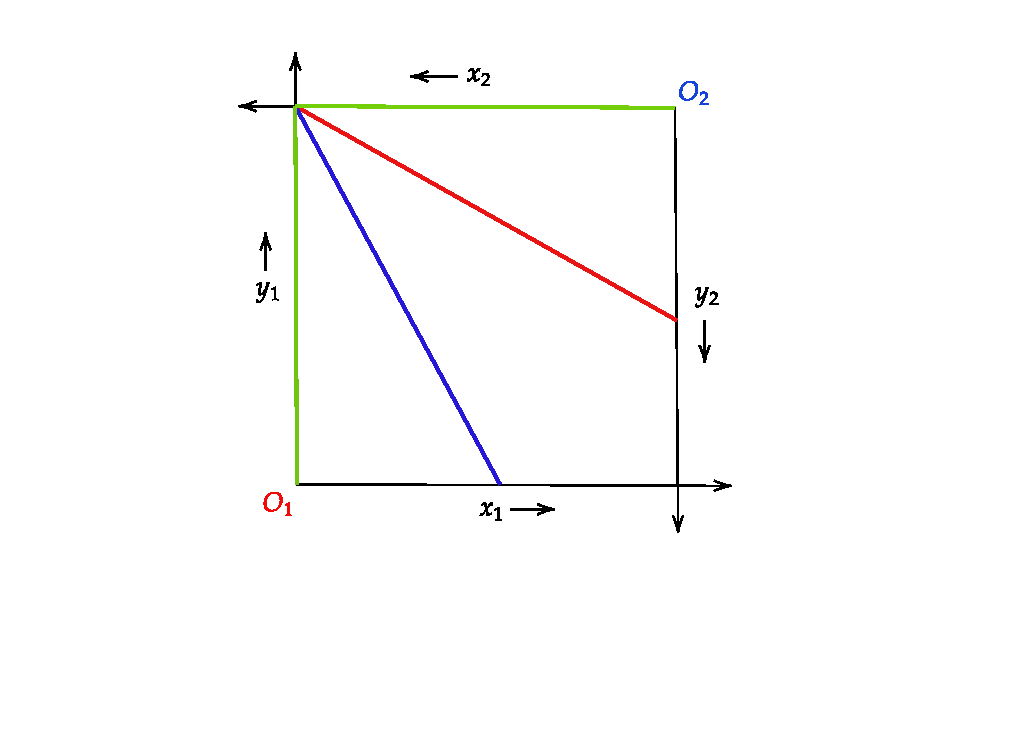
\includegraphics[scale=0.6]{Edge1}
        \caption{Edgeworth Box in Question 1}
        \label{Label}
    \end{figure}
  \end{center}

  \textbf{\underline{NOTE:}}
  In this particular economy if we had the alternate version of the feasibility we will have the same set of Pareto efficient allocations because of the positive externalities in this particular question!

  \subsubsection*{\underline{Competitive Equilibrium}}
  It consists of \(\left( p_{x}^*, p_{y}^* \right) \)   and an allocation \(\left( (x_{1}^*,y_{1}^*),(x_{2}^*,y_{2}^*) \right) \)  such that
    
  \begin{enumerate}
   \item Given \(\left( p_{x}^*,p_{y}^* \right) \),
     
  given, \(\left( x_{2}^*,y_{2}^*  \right) \),

     \(\left( x_{1}^*,y_{1}^*  \right) \) solves;
  \begin{align*}
      \max_{(x_{1},y_{1}) \in \mathbb{R}^2_{+}} & u_{1}(x_{1},y_{1},x_{2}^*,y_{2}^*) \\
      s.t. & p_{x}^*x_{1}+p_{y}^*y_{1} \leq p_{x}^* \omega _{1}^X + p_{y}^*\omega_{1}^Y\\
  \end{align*}     
  and given \(\left( x_{1}^*,y_{1}^*  \right) \),

    \(\left( x_{2}^*,y_{2}^*  \right) \) solves;
  \begin{align*}
    \max_{(x_{2},y_{2}) \in \mathbb{R}^2_{+}} & u_{2}(x_{2},y_{2},x_{1}^*,y_{1}^*) \\
    s.t. & p_{x}^*x_{2}+p_{y}^*y_{2} \leq p_{x}^* \omega _{2}^X + p_{y}^*\omega_{2}^Y\\
\end{align*}       

Alternatively, 
\(\left( (x_{1}^*,y_{1}^*),(x_{2}^*,y_{2}^*) \right) \)  is the Nash Equilibrium of the following demand game;
\begin{itemize}
    \item Set of Players $\{1,2\}$
    \item Action Sets; 
    \begin{align*}
    A_{1}&=\{(x_{1},y_{1}) \in \mathbb{R}^{2}_{+} | p_{x}^*x_{1} + p_{y}^*y_{1} \leq p_{x}^*\omega_{1}^X + \omega_{1}^Y\}\\
    A_{2}&=\{(x_{2},y_{2}) \in \mathbb{R}^{2}_{+} | p_{x}^*x_{2} + p_{y}^*y_{2} \leq p_{x}^*\omega_{2}^X + \omega_{2}^Y\} \\
    \end{align*}
    \item Payoffs;
    \begin{align*}
        u_{1}&: A_{1} \times A_{2} \rightarrow \mathbb{R} \qquad u_{1}(x_{1},y_{1},x_{2},y_{2})\\
        u_{2}&: A_{1} \times A_{2} \rightarrow \mathbb{R} \qquad u_{2}(x_{1},y_{1},x_{2},y_{2})\\
    \end{align*}
    \end{itemize}
    \item Total demand equals total supply in the economy;
    \begin{equation*}
        \begin{split}
            x_{1}^*+x_{2}^*=\omega_{1}^X+\omega_{2}^X\\
            y_{1}^*+y_{2}^*=\omega_{1}^Y+\omega_{2}^Y\\
        \end{split}
    \end{equation*}
  \end{enumerate}

\subsubsection*{Question 2}
Find the set of all Pareto Efficient allocations and the Competitive equilibrium;

\begin{equation*}
    \begin{split}
        \mathcal{F}_{1}= \{\left( (x_{1},y_{1}),(x_{2},y_{2}) \right) \in \mathbb{R}^2_{+} \times \mathbb{R}^2_{+} | x_{1}+x_{2}=2, y_{1}+y_{2}= 2 \}\\
        \mathcal{F}_{2}= \{\left( (x_{1},y_{1}) , (x_{2},y_{2}) \right) \in \mathbb{R}^2_{+} \times \mathbb{R}^2_{+} | x_{1}+x_{2}\leq 2 , y_{1}+y_{2}\leq 2\}\\ 
    \end{split}
\end{equation*}

\begin{align*}
    u_{1}&=(x_{1},y_{1},x_{2},y_{2})= x_{1}+y_{1}-x_{2} \qquad &(2,0) \\
    u_{2}&=(x_{1},y_{1},x_{2},y_{2})= x_{2} \qquad &(0,2)\\ 
\end{align*}
The set of all Pareto efficient allocations is; \(PE_{1}=PE_{2}\) ; 
\[PE_{1}=\{\left( (x_{1},y_{1})(x_{2},y_{2}) \right) \in \mathcal{F}_{1} |y_{2}=0\} \]
\[PE_{2}=\{\left( (x_{1},y_{1})(x_{2},y_{2}) \right) \in \mathcal{F}_{2} |y_{2}=0, y_{1}=2, x_{1}+x_{2}=2\} \]    

The Competitive equilibrium is;
\(CE= ((0,2),(2,0))\) at \(p_{x}=p_{y}=1\)

Now is there any allocation like
\(\left( (x_{1},2),(x_{2},0) \right) \) such that \(x_{1}+x_{2} < 2 \) and \(\left( (x_{1},2),(x_{2},0) \right) \)  is Pareto Efficient in then \(\mathcal{F}_{2}\)? 

\begin{center}
    \begin{figure}[h]
        \centering
        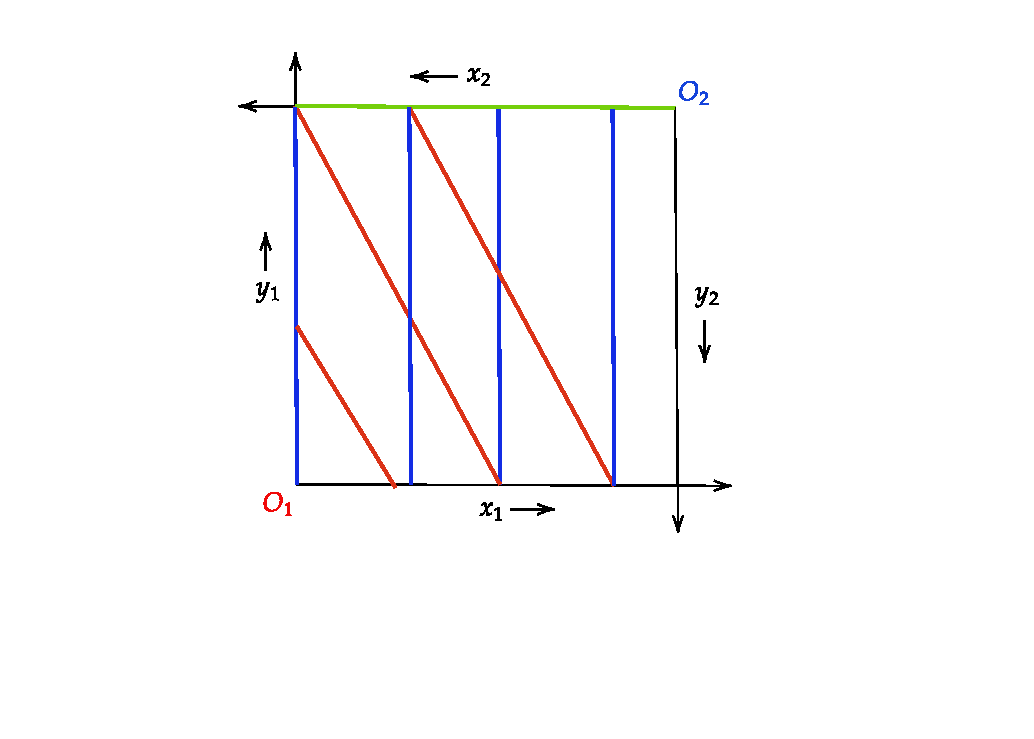
\includegraphics[scale=0.6]{Edge2}
        \caption{Edgeworth Box in Question 2}
        \label{Label}
    \end{figure}
\end{center}

NO! Because if we define \(\epsilon = 2-x_{1}-x_{2}\) and then if we increase the amount of \(x_{1}\) by \(\frac{2\epsilon}{3}\) and \(x_{2}\) by \(\frac{\epsilon}{3}      \) Then utilities of both individuals will increase and therefore any such allocation where \(x_{1}+x_{2}<2\) will not be Pareto Efficient.  

\subsubsection*{Question 3}
Find the set of all Pareto Efficient allocations and also find the Competitve equilibrium;
\begin{align*}
    u_{1}(x_{1},y_{1},x_{2},y_{2})&= x_{1}+ 2\sqrt{y_{1}} \quad &(2,0) \\
    u_{2}(x_{1},x_{2},y_{1},y_{2})&= x_{2} + 2\sqrt{\max(0,2-y_{1})} \quad &(0,2)\\
    \vspace{5pt}
    u_{1}^{ADJ}(x_{1},y_{1})&= x_{1}+2\sqrt{y_{1}} \\
    u_{2}^{ADJ}(x_{2},y_{2})&= x_{2}+2\sqrt{y_{2}} \\
\end{align*}

So the set of all Pareto Efficient allocations is;
\begin{equation*}
    PE=\{\left( (x_{1},y_{1})(x_{2},y_{2}) \right) \in \mathcal{F} | (y_{1}=y_{2}=1) \ \vee \ (x_{1}=0 \ \wedge \ y_{1}\leq 1) \ \vee \ (x_{2}=0 \ \wedge \ y_{2}\leq 1)\}
\end{equation*}
and the Competitive equilibrium is 
\begin{equation*}
    CE=\left( \left( \frac{P_{X}}{P_{Y}}=\sqrt{2}, \right),\left( (2-\sqrt{2}, 2),(\sqrt{2},0) \right) \right)  
\end{equation*}   

\begin{center}
    \begin{figure}[h]
        \centering
        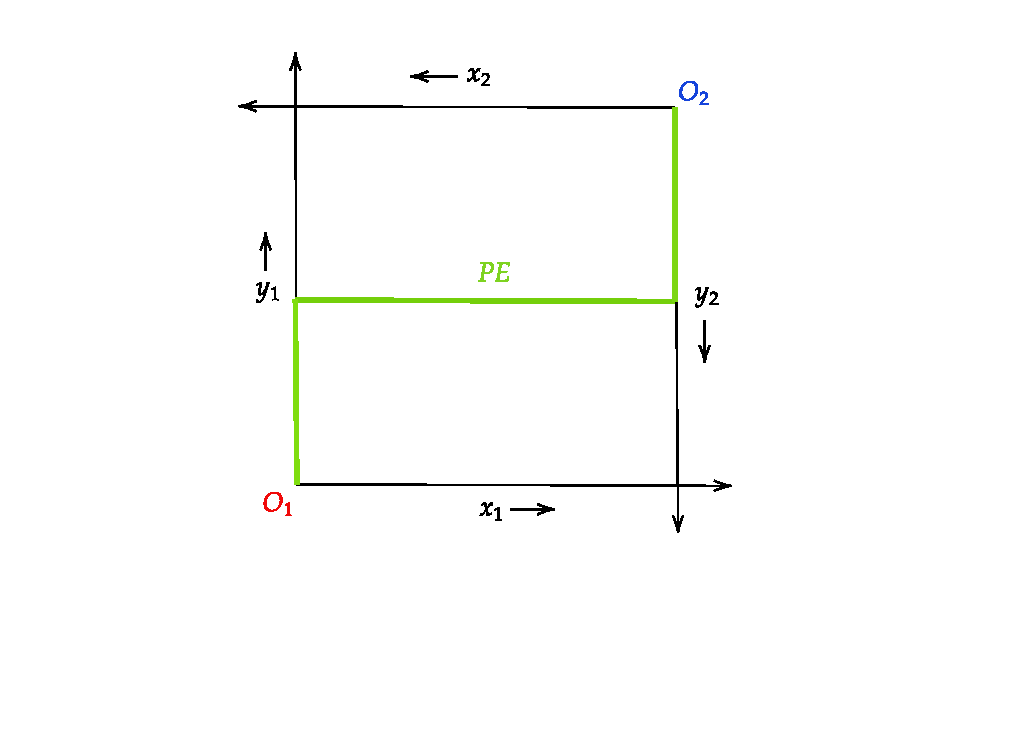
\includegraphics[scale=0.6]{Edge3}
        \caption{Edgeworth Box In Question 3}
        \label{Label}
    \end{figure}
    
\end{center}

\subsubsection*{Question 4}

\begin{align*}
    u_{1}(x_{1},y_{1},x_{2},y_{2})&=\max(x_{1},y_{1},x_{2},y_{2}) \quad &(3,3)\\
    u_{2}(x_{1},y_{1},x_{2},y_{2})&= x_{2}+y_{2} \quad &(1,1)\\
\end{align*}
 \(PE=\left( (0,0),(4,4) \right) \) 
 
 \(CE=\text{DNE} \)  
 \begin{center}
    \begin{figure}[ht!]
        \centering
        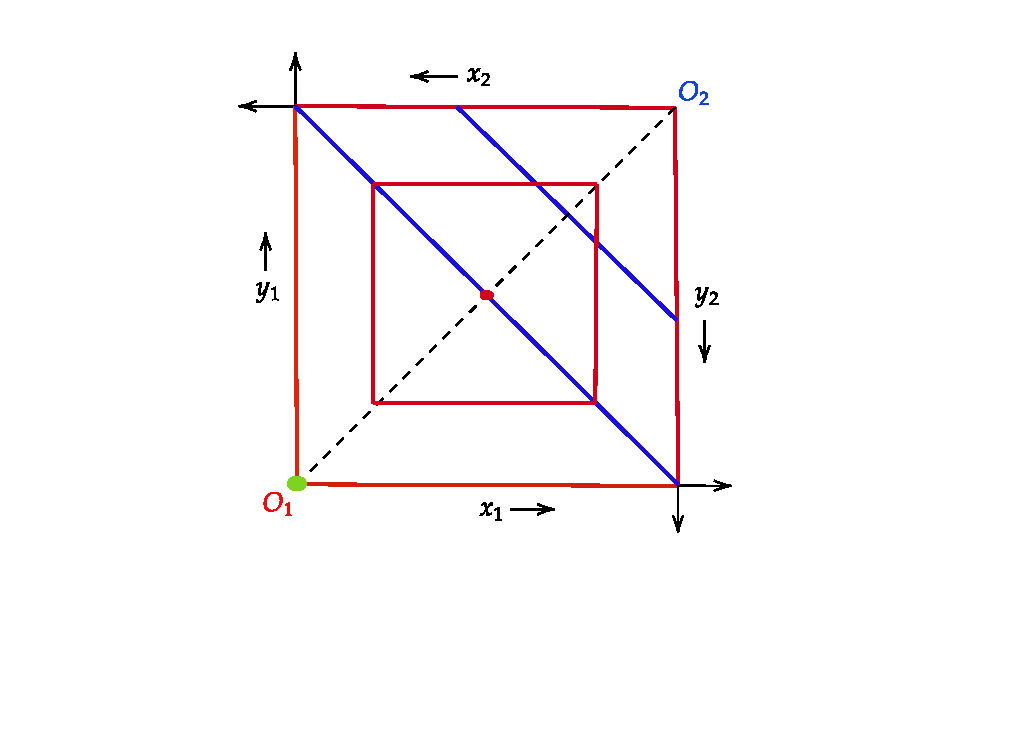
\includegraphics[scale=0.4]{Edge4}
        \caption{Edgewoth Box in Question 4}
        \label{Label}
    \end{figure}
    
 \end{center}
\end{document}